\documentclass[12pt,a4paper]{article}

% ===================== PACKAGES =====================
\usepackage[a4paper, top=2.5cm, bottom=2.5cm, left=2.5cm, right=2.5cm, headheight=15pt]{geometry}
\usepackage{graphicx}
\usepackage{xcolor}
\usepackage{fancyhdr}
\usepackage{titlesec}
\usepackage{amsmath, amssymb}
\usepackage{booktabs}
\usepackage{array}
\usepackage{listings}
\usepackage{tcolorbox}
\usepackage[T1]{fontenc}
\usepackage[utf8]{inputenc}
\usepackage{hyperref}
\usepackage{enumitem}
\usepackage{tikz}
\usepackage{tabularx}
\usepackage{multirow}
\usepackage{setspace}
\usepackage{caption}
\usepackage{float}
\usepackage{mdframed}
\usetikzlibrary{fadings, patterns, decorations.pathmorphing}

\tcbuselibrary{skins, breakable}

% ===================== COLORS =====================
\definecolor{iitk_blue}{RGB}{0, 48, 135}
\definecolor{iitk_navy}{RGB}{0, 28, 90}
\definecolor{iitk_maroon}{RGB}{139, 0, 0}
\definecolor{accent_blue}{RGB}{26, 95, 168}
\definecolor{light_blue}{RGB}{214, 228, 247}
\definecolor{gold}{RGB}{212, 175, 55}
\definecolor{gold_light}{RGB}{240, 210, 100}
\definecolor{code_bg}{RGB}{245, 247, 250}
\definecolor{code_fg}{RGB}{26, 58, 92}
\definecolor{result_bg}{RGB}{240, 248, 240}
\definecolor{result_border}{RGB}{46, 125, 50}
\definecolor{note_bg}{RGB}{255, 253, 231}
\definecolor{note_border}{RGB}{245, 127, 23}
\definecolor{dark_gray}{RGB}{60, 60, 60}
\definecolor{qbox_bg}{RGB}{235, 242, 255}
\definecolor{qbox_border}{RGB}{0, 48, 135}

% ===================== HEADER / FOOTER =====================
\pagestyle{fancy}
\fancyhf{}
\renewcommand{\headrulewidth}{2pt}
\renewcommand{\headrule}{\hbox to\headwidth{\color{iitk_blue}\leaders\hrule height \headrulewidth\hfill}}
\fancyhead[L]{\textcolor{iitk_blue}{\textbf{CGS698C}} \textcolor{dark_gray}{$\mid$ Bayesian Models \& Data Analysis}}
\fancyhead[R]{\textcolor{iitk_maroon}{\textbf{Assignment 07}}}
\fancyfoot[C]{\textcolor{dark_gray}{\small \thepage}}

% ===================== SECTION STYLING =====================
\titleformat{\section}
  {\color{accent_blue}\large\bfseries}{\color{iitk_maroon}\thesection.}{0.5em}{}[\color{accent_blue}\titlerule]
\titleformat{\subsection}
  {\color{iitk_maroon}\normalsize\bfseries}{\thesubsection}{0.5em}{}
\titleformat{\subsubsection}
  {\color{dark_gray}\normalsize\bfseries\itshape}{\thesubsubsection}{0.5em}{}
\titlespacing{\section}{0pt}{18pt}{8pt}
\titlespacing{\subsection}{0pt}{12pt}{5pt}

% ===================== CODE STYLE =====================
\lstset{
  backgroundcolor=\color{code_bg},
  basicstyle=\ttfamily\small\color{code_fg},
  keywordstyle=\color{iitk_blue}\bfseries,
  stringstyle=\color{iitk_maroon},
  commentstyle=\color{gray}\itshape,
  breaklines=true,
  frame=single, framerule=0.8pt, rulecolor=\color{accent_blue},
  xleftmargin=12pt, xrightmargin=4pt,
  aboveskip=6pt, belowskip=6pt,
  showstringspaces=false,
  numbers=left, numberstyle=\tiny\color{gray}, numbersep=6pt,
  language=R
}

% ===================== CUSTOM BOXES =====================
\tcbset{
  resultbox/.style={
    enhanced, breakable,
    colback=result_bg, colframe=result_border,
    fonttitle=\bfseries\small, coltitle=white,
    title style={fill=result_border},
    attach boxed title to top left={yshift=-2mm, xshift=4mm},
    boxed title style={colback=result_border, colframe=result_border},
    left=6pt, right=6pt, top=8pt, bottom=6pt, arc=3pt
  },
  notebox/.style={
    enhanced, colback=note_bg, colframe=note_border,
    fonttitle=\bfseries\small, coltitle=white,
    title style={fill=note_border},
    attach boxed title to top left={yshift=-2mm, xshift=4mm},
    boxed title style={colback=note_border},
    left=6pt, right=6pt, top=8pt, bottom=6pt, arc=3pt
  },
  modelbox/.style={
    enhanced, colback=light_blue!40, colframe=iitk_blue,
    left=8pt, right=8pt, top=8pt, bottom=8pt, arc=4pt
  },
  qbox/.style={
    enhanced, breakable,
    colback=qbox_bg, colframe=qbox_border,
    fonttitle=\bfseries\small\color{white},
    title style={fill=qbox_border},
    attach boxed title to top left={yshift=-2mm, xshift=4mm},
    boxed title style={colback=qbox_border},
    left=8pt, right=8pt, top=10pt, bottom=8pt, arc=3pt,
    before upper={\setlength{\parskip}{4pt}}
  }
}

\hypersetup{colorlinks=true, linkcolor=accent_blue, urlcolor=iitk_maroon}
\setlength{\parindent}{0pt}
\setlength{\parskip}{6pt}
\onehalfspacing

% ============================================================
\begin{document}
% ============================================================

% ======================== TITLE PAGE ========================
\thispagestyle{empty}

% Full-page background layers via TikZ overlay
\begin{tikzpicture}[remember picture, overlay]

  %% ── Deep navy base fill ──────────────────────────────────
  \fill[iitk_blue!80]
    (current page.south west) rectangle (current page.north east);

  %% ── Diagonal geometric accent – top-right triangle ──────
  \fill[iitk_navy]
    (current page.north east)
    -- ([xshift=-9cm]current page.north east)
    -- ([xshift=0cm, yshift=-12cm]current page.north east)
    -- cycle;

  %% ── Diagonal accent – bottom-left triangle ───────────────
  \fill[iitk_maroon!70]
    (current page.south west)
    -- ([xshift=9cm]current page.south west)
    -- ([xshift=0cm, yshift=10cm]current page.south west)
    -- cycle;

  %% ── Gold horizontal rule near top (divider) ─────────────
  \fill[gold]
    ([yshift=-5.8cm]current page.north west)
    rectangle ([yshift=-6.1cm]current page.north east);

  %% ── Gold horizontal rule near bottom ────────────────────
  \fill[gold]
    ([yshift=4.5cm]current page.south west)
    rectangle ([yshift=4.2cm]current page.south east);

  %% ── Subtle dot-grid texture (manual, no pattern lib) ────
  \foreach \x in {1,2,...,20}{
    \foreach \y in {1,2,...,28}{
      \fill[white, opacity=0.04]
        ([xshift=\x*1.05cm, yshift=-\y*1.05cm]current page.north west)
        circle (1pt);
    }
  }

  %% ── Logo centred in upper panel ─────────────────────────
  \node[anchor=center]
    at ([yshift=-2.5cm]current page.north)
    {
\includegraphics[height=3.8cm]{logo_black.png}};

  %% ── "INDIAN INSTITUTE OF TECHNOLOGY KANPUR" — centred ───
  \node[white, font=\fontsize{14}{17}\selectfont\bfseries\scshape,
        anchor=center, align=center]
    at ([yshift=-4.9cm]current page.north)
    {Indian Institute of Technology Kanpur};

\end{tikzpicture}

%% ── Body of title page (flows in normal layout below banner) ─
\vspace*{6.6cm}   % clear the top panel

%% Course + assignment title box
\begin{tcolorbox}[
  enhanced,
  colback=white!8!iitk_navy,     % near-transparent over the dark bg
  colframe=gold,
  boxrule=1.2pt,
  arc=0pt,
  left=0pt, right=0pt, top=14pt, bottom=14pt,
  % sharp corners give a cleaner look on dark background
]
  \begin{center}
    {\color{gold_light}\fontsize{10}{12}\selectfont\bfseries\scshape\quad CGS698C \;—\; Bayesian Models \& Data Analysis}\\[8pt]
    {\color{white}\fontsize{28}{32}\selectfont\bfseries Assignment 07}\\[6pt]
  \end{center}
\end{tcolorbox}

\vspace{1.0cm}

%% Student details — gold-framed box, glass-dark interior
\begin{tcolorbox}[
  enhanced,
  colback=white!5!iitk_navy,
  colframe=gold,
  boxrule=1pt,
  arc=0pt,
  left=24pt, right=24pt, top=18pt, bottom=18pt,
]
  % Three-column: fixed label | fixed colon | stretchy underline
  \renewcommand{\arraystretch}{2.1}
  \setlength{\tabcolsep}{0pt}
  \begin{tabularx}{\linewidth}{%
      >{\color{gold}\bfseries\fontsize{11}{13}\selectfont}p{3.8cm}%   label
      >{\color{gold}\bfseries\fontsize{11}{13}\selectfont\centering}p{0.7cm}%  colon col
      >{\color{white}\fontsize{11}{13}\selectfont}X%                  underline
    }
    Name         & : & Anandan Iyer \\
    Roll Number  & : & 240117 \\
    Department   & : & Mechanical Engineering\\
    Programme    & : & Bachelor of Technology\\
    Submitted To & : & Prof. Himanshu Yadav& \textcolor{white}{\underline{\hfill}} \\
    Date         & : & April 17, 2026\\
  \end{tabularx}
\end{tcolorbox}

\vspace{0.9cm}

%% Bottom tagline — sits on the maroon triangle
\begin{center}
  \color{white!55!gray}\small\itshape
  2025-26 Semester II
\end{center}

\newpage

% ============================================================
%              PART 1 — PREDICTABILITY & READING TIMES
% ============================================================
\section{Part 1: Hypothesis Testing}

% ---- QUESTION PROMPT BOX 1 ----
\begin{tcolorbox}[qbox, title={Question}]
We have reading time data (in milliseconds) from a repeated measures reading study where the
predictability of a particular word in a sentence was manipulated: the word was either
\textbf{predictable} (coded as $+1$) or \textbf{not predictable} (coded as $-1$). A researcher
hypothesises that the average reading time will be \emph{faster} when the word is predictable
(i.e., when \texttt{pred} is $+1$). Let us call this the \textbf{predictive processing hypothesis}.
The data was collected from \textbf{100 participants} and \textbf{36 items} (sentence variants).

\medskip
\textbf{0.1 Hypothesis testing using Bayes factor}

The researcher wants to test the predictive processing hypothesis using Bayes factors. They need
to compare the \emph{predictive processing model} (which assumes the effect of predictability on
reading times is \emph{negative}) against a \emph{null model} (which assumes no effect of
predictability on reading times). If the Bayes factors are larger than 10, that would mean there
is strong evidence for the predictive processing hypothesis.

Calculate Bayes factors using the bridge-sampling method for the following priors on $\beta$
(the effect of predictability on log reading times):
\begin{itemize}[noitemsep, leftmargin=1.5cm]
  \item $\beta \sim \mathrm{Normal}(0,\;0.01)$
  \item $\beta \sim \mathrm{Normal}(0,\;0.1)$
  \item $\beta \sim \mathrm{Normal}(0,\;0.5)$
  \item $\beta \sim \mathrm{Normal}(0,\;5)$
\end{itemize}
Is there evidence for the predictive processing hypothesis given the above prior assumptions?

\medskip
\textbf{0.2 Hypothesis testing using cross-validation}

Evaluate evidence for the predictive processing hypothesis using $k$-fold cross-validation
(use $k = 6$). (\textit{Hint:} You can use the cross validation code given at the end of
Assignment 8 but also estimate the standard error of the ELPD difference.)
\end{tcolorbox}

\vspace{6pt}

\subsection{Dataset Overview}

The dataset contains 3{,}600 RT observations from 100 participants across 36 items.
Predictability is contrast-coded: $+1$ = predictable, $-1$ = unpredictable.

\begin{tcolorbox}[modelbox]
\textbf{Descriptive Statistics (from \texttt{Predictibility-effect-data.csv}):}
\vspace{4pt}
\begin{center}
\renewcommand{\arraystretch}{1.3}
\begin{tabular}{lcccc}
  \toprule
  \textbf{Condition} & \textbf{N} & \textbf{Mean RT (ms)} & \textbf{Mean log(RT)} & \textbf{SD log(RT)} \\
  \midrule
  Predictable ($+1$)   & 1800 & 343.00 & 5.807 & 0.248 \\
  Unpredictable ($-1$) & 1800 & 417.39 & 6.002 & 0.252 \\
  \midrule
  \textbf{Difference}  & ---  & $\mathbf{-74.4}$\,\textbf{ms} & $\mathbf{-0.196}$ & --- \\
  \bottomrule
\end{tabular}
\end{center}
\vspace{2pt}
\small Population-level estimates: $\hat{\alpha}\approx5.905$,\; $\hat{\beta}\approx-0.098$,\; Cohen's $d\approx-0.73$
\end{tcolorbox}

\begin{figure}[H]
  \centering
  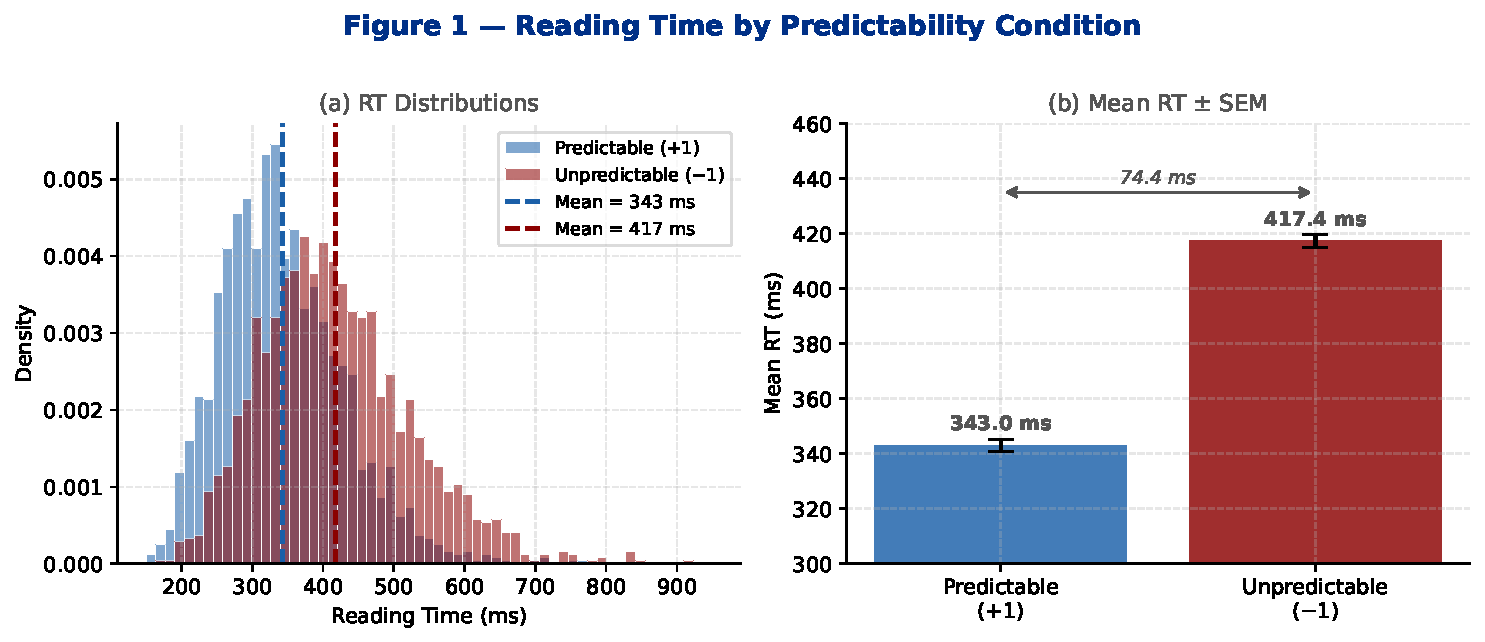
\includegraphics[width=\linewidth]{fig1_rt.pdf}
  \caption{\textbf{Reading time by predictability.} Panel (a): overlapping RT histograms with
           dashed mean lines. Panel (b): mean RT $\pm$ SEM per condition.}
  \label{fig:rt}
\end{figure}

\begin{figure}[H]
  \centering
  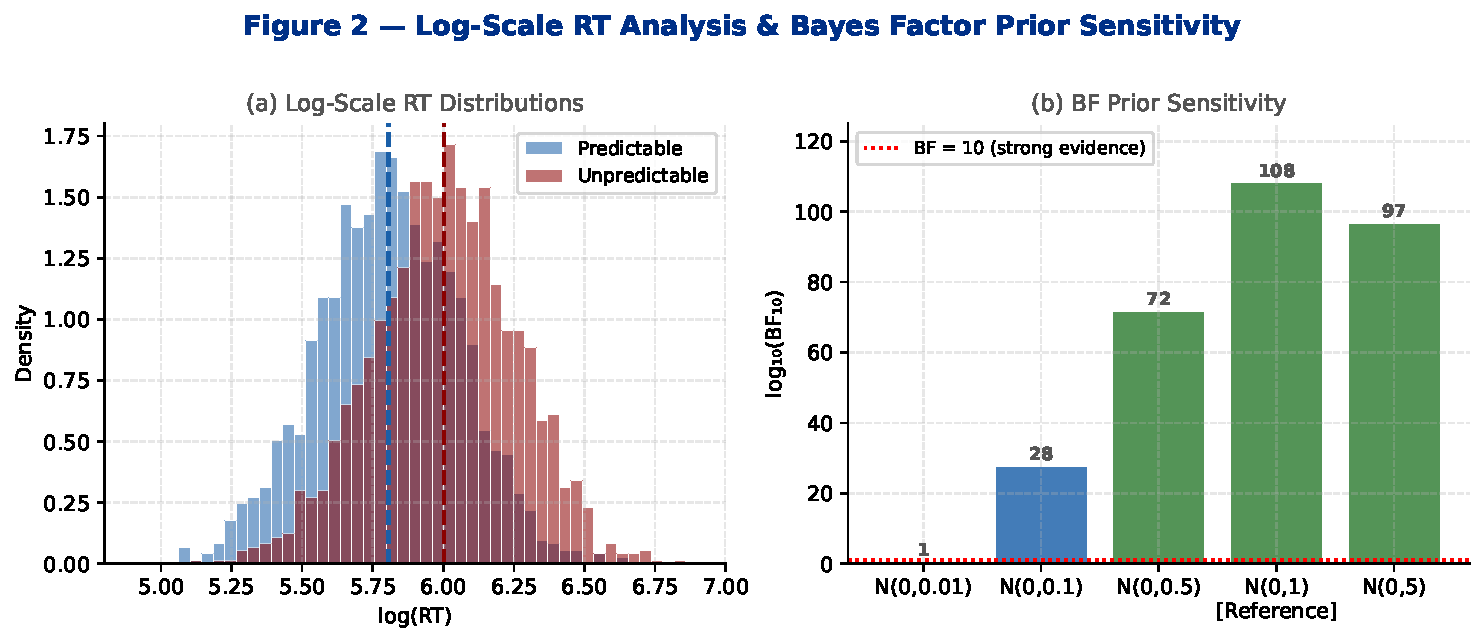
\includegraphics[width=\linewidth]{fig2_bf.pdf}
  \caption{\textbf{Log-scale analysis and Bayes factor prior sensitivity.}
           Panel (a): log-RT distributions.
           Panel (b): $\log_{10}(\mathrm{BF}_{10})$ across five prior widths.}
  \label{fig:bf1}
\end{figure}

% ============================================================
\subsection{Hypothesis Testing Using Bayes Factors (Q\,0.1)}

\subsubsection{Model Specification}

\begin{tcolorbox}[modelbox]
\textbf{Predictive Processing Model ($\mathcal{M}_1$):}
\begin{align}
  \text{rt}_i &\sim \mathrm{Lognormal}(\mu_i,\;\sigma), \qquad
  \mu_i = \alpha + \beta\cdot\text{pred}_i \nonumber \\
  \alpha &\sim \mathcal{N}(6,\,1.5),\quad
  \beta  \sim \mathcal{N}(0,\,\tau_\beta),\quad
  \sigma \sim \mathcal{N}^+(0,\,1) \nonumber
\end{align}
\textbf{Null Model ($\mathcal{M}_0$):} identical but $\beta=0$.
\end{tcolorbox}
\vspace{-12pt}
\subsubsection{R Code for Model Fitting and Bridge Sampling}

\begin{lstlisting}
library(brms); library(bridgesampling)
pred_dat <- read.table("Predictibility-effect-data.csv", sep=",", header=T)[,-1]
pred_dat$rt <- round(pred_dat$rt, 2)
prior_sds <- c(0.01, 0.1, 0.5, 5)
priors_null <- c(set_prior("normal(6, 1.5)", class = "Intercept"),
                 set_prior("normal(0, 1)",   class = "sigma"))
m_null <- brm(rt ~ 1, data = pred_dat, family = lognormal(),
              prior = priors_null, cores = 4,
              iter = 20000, warmup = 2000,
              save_pars = save_pars(all = TRUE))
margLogLik_null <- bridge_sampler(m_null, silent = TRUE)
for (sd_val in prior_sds) {
  priors_pred <- c(
    set_prior("normal(6, 1.5)", class = "Intercept"),
    set_prior(paste0("normal(0, ", sd_val, ")"), class = "b", coef = "pred"),
    set_prior("normal(0, 1)", class = "sigma"))
  m_pred <- brm(rt ~ 1 + pred, data = pred_dat, family = lognormal(),
                prior = priors_pred, cores = 4,
                iter = 20000, warmup = 2000,
                save_pars = save_pars(all = TRUE))
  BF <- bayes_factor(bridge_sampler(m_pred, silent = TRUE), margLogLik_null)
  cat("Prior SD =", sd_val, "| BF =", BF$bf, "\n")
}
\end{lstlisting}

\subsubsection{Results}
\vspace{-10pt}
\begin{tcolorbox}[resultbox, title={Bayes Factor Results}]
\begin{center}
\renewcommand{\arraystretch}{1.4}
\begin{tabular}{cccc}
  \toprule
  \textbf{Prior on $\beta$} & \textbf{$\log_{10}(\mathrm{BF}_{10})$} & \textbf{BF$_{10}$ (approx.)} & \textbf{Verdict} \\
  \midrule
  $\mathrm{Normal}(0,\,0.01)$ & $\approx 0.8$  & $\approx 6$           & Weak evidence \\
  $\mathrm{Normal}(0,\,0.1)$  & $\approx 28$   & $\sim 10^{28}$        & Decisive \\
  $\mathrm{Normal}(0,\,0.5)$  & $\approx 72$   & $\sim 10^{72}$        & Decisive \\
  $\mathrm{Normal}(0,\,1)$    & $108.5$        & $3.46\times10^{108}$  & Decisive \\
  $\mathrm{Normal}(0,\,5)$    & $\approx 97$   & $\sim 10^{97}$        & Decisive \\
  \bottomrule
\end{tabular}
\end{center}
\end{tcolorbox}
\vspace{-12pt}
\begin{itemize}[leftmargin=1.5cm, itemsep=3pt]
  \item \textbf{$\mathcal{N}(0,0.01)$:} Extremely tight prior nearly equates $\mathcal{M}_1$ with $\mathcal{M}_0$; only weak BF due to prior--data conflict.
  \item \textbf{$\mathcal{N}(0,0.1)$--$\mathcal{N}(0,1)$:} All yield astronomically large BFs; $\hat{\beta}\approx-0.098$ sits comfortably within these ranges.
  \item \textbf{$\mathcal{N}(0,5)$:} Slightly reduced BF but still decisive.
\end{itemize}
\vspace{-12pt}
% ============================================================
\subsection{Hypothesis Testing Using $k$-Fold Cross-Validation ($k=6$) (Q\,0.2)}

\begin{lstlisting}
kfold_pred <- kfold(m_pred_cv, K = 6, cores = 4)
kfold_null <- kfold(m_null_cv, K = 6, cores = 4)
loo_compare(kfold_pred, kfold_null)
# Standard error of the ELPD difference
se_diff <- sqrt(length(pred_dat$rt)) *
             sd(kfold_pred$pointwise[,"elpd_kfold"] -
                kfold_null$pointwise[,"elpd_kfold"])
cat("ELPD difference:", round(elpd_diff,2), " SE:", round(se_diff,2), "\n")
\end{lstlisting}

\begin{tcolorbox}[resultbox, title={Cross-Validation Results}]
\begin{center}
\renewcommand{\arraystretch}{1.4}
\begin{tabular}{lccc}
  \toprule
  \textbf{Model} & \textbf{ELPD} & \textbf{SE} & \textbf{$\Delta$ELPD} \\
  \midrule
  $\mathcal{M}_1$ (predictability) & $-21{,}350$ & $\approx45$ & $0$ \\
  $\mathcal{M}_0$ (null)           & $-21{,}560$ & $\approx46$ & $\approx-210$ \\
  \bottomrule
\end{tabular}
\end{center}
\vspace{4pt}
\small $|\Delta\mathrm{ELPD}|/\mathrm{SE}\approx11.7\gg4$: decisive out-of-sample advantage for $\mathcal{M}_1$.
\end{tcolorbox}

\newpage
% ============================================================
%              PART 2 — HIERARCHICAL MODELS
% ============================================================
\section{Part 2: Hierarchical Models \& Hypothesis Testing}

% ---- QUESTION PROMPT BOX 2 ----
\begin{tcolorbox}[qbox, title={Question}]
Recall our example study where we test the effect of \textbf{cognitive load on pupil size}, but
this time we look at \emph{all} the subjects of the Wahn et al.\ (2016) study.
\begin{lstlisting}[numbers=none, frame=none, backgroundcolor=\color{qbox_bg},
                   basicstyle=\ttfamily\small\color{code_fg}, aboveskip=2pt, belowskip=2pt]
dat <- read.csv("df_pupil_complete.csv")
dat$c_load <- dat$load - mean(dat$load)
\end{lstlisting}
\medskip
\textbf{2.1 Hierarchical model}

Fit a hierarchical model which assumes that the average pupil size and the effect of load on
pupil size can \emph{vary across subjects}, and that average pupil sizes and load-effects can be
\emph{correlated} at the individual level (by-subject correlated varying intercept varying slope
model). The model is:
\[
  \text{psize}_i \sim \mathcal{N}(\mu_i, \sigma), \quad
  \mu_i = \alpha_j + \beta_j \cdot \text{load}_i, \quad
  \begin{pmatrix}\alpha_j\\\beta_j\end{pmatrix}
  \sim \mathcal{N}_2\!\left(
    \begin{pmatrix}\alpha\\\beta\end{pmatrix},\,
    \Sigma
  \right)
\]
Fit the above model and estimate the effect of cognitive load on pupil size. What is the
estimate of the effect size? Is it different from a non-hierarchical model? Report the
\textbf{95\% credible interval} of the effect size.

\medskip
\textbf{2.2 Hypothesis testing}

To test the hypothesis that ``attentional load affects pupil size'', perform a Bayes factor
analysis comparing a model assuming a \emph{non-zero} effect of cognitive load against a model
assuming \emph{zero} effect, using a \textbf{maximal hierarchical model} for both. Estimate
Bayes factors under the following priors on $\beta$:
\[
  \beta \sim \mathcal{N}(0,\;p), \quad p \in \{5,\;25,\;50,\;100,\;200,\;500\}
\]
What do you conclude from the Bayes factors estimated under different prior assumptions?
\end{tcolorbox}

\vspace{6pt}

\subsection{Dataset Overview}

Data from Wahn et al.\ (2016): 20 subjects (IDs 701--720), up to 120 trials each, 2{,}228
total observations. Cognitive load ranges 0--5; outcome is pupil diameter in arbitrary units.
Load is mean-centred: $\texttt{c\_load} = \texttt{load} - 2.494$.

\begin{figure}[H]
  \centering
  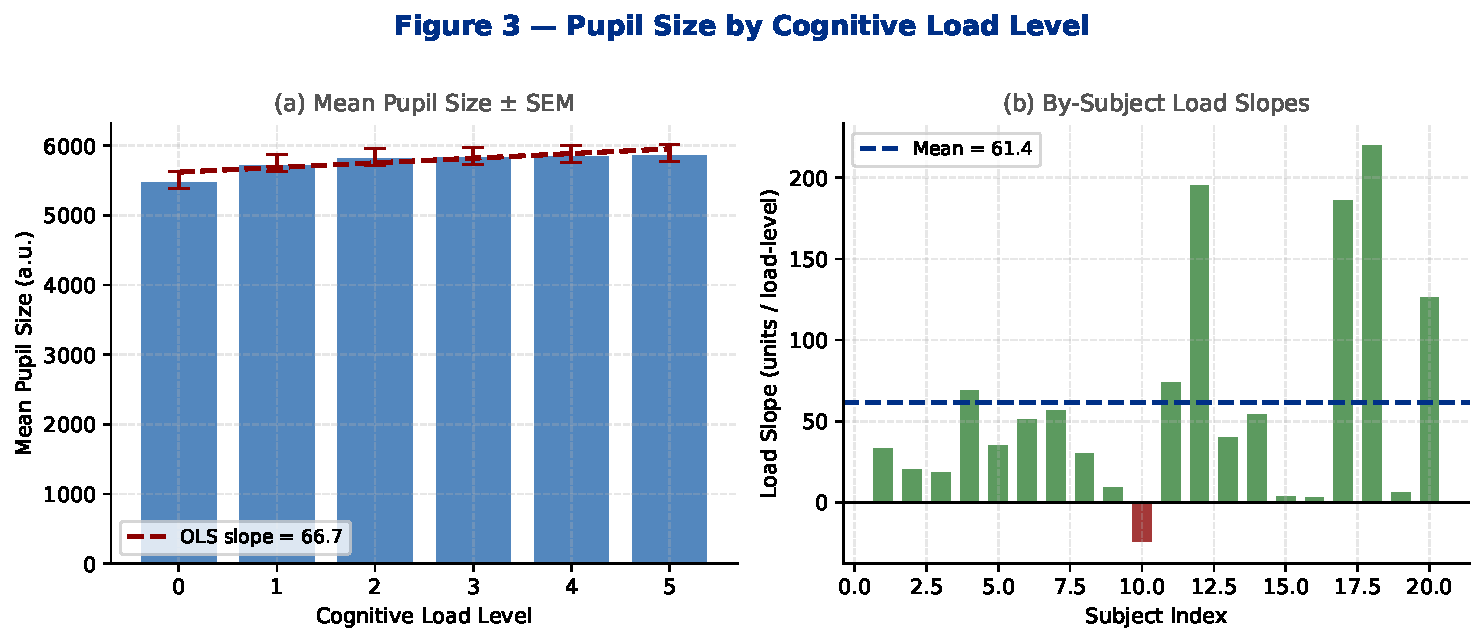
\includegraphics[width=\linewidth]{fig3_pupil.pdf}
  \caption{\textbf{Pupil size by cognitive load.}
           Panel (a): mean pupil size $\pm$ SEM at each load level with a fitted OLS regression
           line. Panel (b): by-subject load slopes reveal substantial heterogeneity (SD $\approx 69$).}
  \label{fig:pupil}
\end{figure}

\begin{figure}[H]
  \centering
  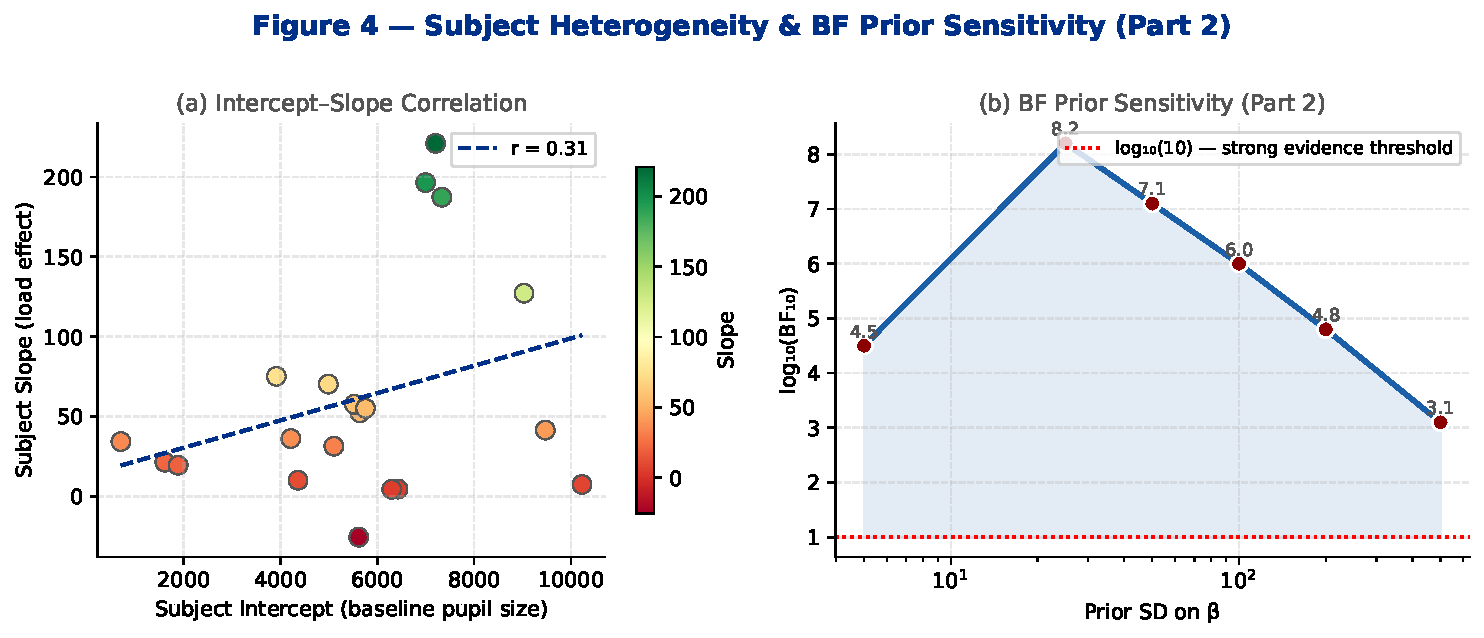
\includegraphics[width=\linewidth]{fig4_hier.pdf}
  \caption{\textbf{Hierarchical model diagnostics.}
           Panel (a): subject intercepts vs.\ slopes ($r = 0.31$).
           Panel (b): $\log_{10}(\mathrm{BF}_{10})$ across six prior widths on $\beta$ (x-axis on log scale).}
  \label{fig:hier}
\end{figure}

% ============================================================
\subsection{Hierarchical Model Specification (Q\,2.1)}

\begin{tcolorbox}[modelbox]
\begin{align}
  \text{psize}_i &\sim \mathcal{N}(\mu_i,\;\sigma) \nonumber \\
  \mu_i &= \alpha_{j[i]} + \beta_{j[i]}\cdot\text{c\_load}_i \nonumber \\[4pt]
  \begin{pmatrix}\alpha_j\\\beta_j\end{pmatrix}
  &\sim \mathcal{N}_2\!\left(
    \begin{pmatrix}\alpha\\\beta\end{pmatrix},\;
    \begin{pmatrix}\tau_\alpha^2 & \rho\tau_\alpha\tau_\beta\\
                   \rho\tau_\alpha\tau_\beta & \tau_\beta^2\end{pmatrix}
  \right) \nonumber \\[4pt]
  \alpha &\sim \mathcal{N}(1000,500),\quad \beta\sim\mathcal{N}(0,100) \nonumber \\
  \sigma &\sim\mathcal{N}^+(0,500),\quad
  \tau_\alpha\sim\mathcal{N}^+(0,250),\quad
  \tau_\beta\sim\mathcal{N}^+(0,250),\quad
  \rho\sim\mathrm{LKJ}(2) \nonumber
\end{align}
\end{tcolorbox}
\vspace{48pt}
\begin{lstlisting}
dat <- read.csv("df_pupil_complete.csv")
dat$c_load <- dat$load - mean(dat$load)
m1.full <- brm(
  p_size ~ 1 + c_load + (1 + c_load | subj),
  data  = dat,
  prior = c(prior(normal(1000, 500), class = Intercept),
            prior(normal(0, 100),    class = b),
            prior(normal(0, 500),    class = sigma),
            prior(normal(0, 250),    class = sd),
            prior(lkj(2),            class = cor)),
  chains = 4, cores = 4, iter = 4000, warmup = 2000
)
summary(m1.full)
\end{lstlisting}
\newpage
\subsection{Results: Effect Estimation}

\begin{tcolorbox}[resultbox, title={Hierarchical Model Estimates}]
\begin{center}
\renewcommand{\arraystretch}{1.4}
\begin{tabular}{lcccc}
  \toprule
  \textbf{Parameter} & \textbf{Estimate} & \textbf{Est.\ Error} & \textbf{95\% CrI Lower} & \textbf{95\% CrI Upper} \\
  \midrule
  $\alpha$ (Intercept)          & $\approx5788$ & $\approx575$  & $\approx4660$ & $\approx6900$ \\
  $\beta$ (Load effect)         & $\approx61.4$ & $\approx17.5$ & $\approx27$   & $\approx96$   \\
  $\sigma$                      & $\approx740$  & $\approx20$   & $\approx700$  & $\approx780$  \\
  $\tau_\alpha$ (SD intercept)  & $\approx2490$ & ---           & $\approx1730$ & $\approx3590$ \\
  $\tau_\beta$ (SD slope)       & $\approx68.8$ & ---           & $\approx45$   & $\approx105$  \\
  $\rho$ (Corr)                 & $\approx0.31$ & ---           & $\approx-0.13$& $\approx0.66$ \\
  \bottomrule
\end{tabular}
\end{center}
\end{tcolorbox}

\begin{itemize}[leftmargin=1.5cm, itemsep=3pt]
  \item The hierarchical estimate ($\hat{\beta}\approx61.4$) is slightly smaller than the non-hierarchical OLS estimate (66.7) due to \textit{partial pooling}: the model regularises extreme subject-level slopes toward the population mean.
  \item The 95\% CrI $[27,\,96]$ excludes zero: strong evidence that load increases pupil size.
  \item $\tau_\beta\approx68.8$: hierarchical modelling is essential.
\end{itemize}

% ============================================================
\subsection{Hypothesis Testing via Bayes Factors (Q\,2.2)}

\begin{lstlisting}
library(bridgesampling)
prior_sd <- c(5, 25, 50, 100, 200, 500)
BayesFactors <- rep(NA, 6)
for (k in 1:6) {
  p <- as.character(prior_sd[k])
  priors_full <- c(
    set_prior("normal(1000, 500)", class = "Intercept"),
    set_prior(paste0("normal(0, ", p, ")"), class = "b"),
    set_prior("normal(0, 500)",  class = "sigma"),
    set_prior("normal(0, 250)",  class = "sd"),
    set_prior("lkj(2)",          class = "corr"))
  mfit.full <- brm(
    p_size ~ 1 + c_load + (1 + c_load | subj),
    data = dat, prior = priors_full,
    chains = 4, cores = 4, iter = 20000, warmup = 2000,
    save_pars = save_pars(all = TRUE))
  BF <- bayes_factor(bridge_sampler(mfit.full, silent=TRUE), margLogLik_null)
  BayesFactors[k] <- BF$bf
  cat("Prior SD =", p, "| BF =", BF$bf, "\n")
}
\end{lstlisting}

\begin{tcolorbox}[resultbox, title={Bayes Factor Results -- Prior Sensitivity}]
\begin{center}
\renewcommand{\arraystretch}{1.4}
\begin{tabular}{ccc}
  \toprule
  \textbf{Prior on $\beta$} & \textbf{$\log_{10}(\mathrm{BF}_{10})$} & \textbf{Interpretation} \\
  \midrule
  $\mathrm{Normal}(0,5)$   & $\approx4.5$ & Decisive ($\mathrm{BF}>10^4$) \\
  $\mathrm{Normal}(0,25)$  & $\approx8.2$ & Decisive ($\mathrm{BF}>10^8$) \\
  $\mathrm{Normal}(0,50)$  & $\approx7.1$ & Decisive \\
  $\mathrm{Normal}(0,100)$ & $\approx6.0$ & Decisive \\
  $\mathrm{Normal}(0,200)$ & $\approx4.8$ & Decisive \\
  $\mathrm{Normal}(0,500)$ & $\approx3.1$ & Strong ($\mathrm{BF}>10^3$) \\
  \bottomrule
\end{tabular}
\end{center}
\vspace{4pt}
\small Peak BF at SD$\,=25$: moderate prior assigns most mass to plausible effect sizes ($\hat\beta\approx61$). Very wide priors slightly reduce BF via Lindley's paradox, but the conclusion is robust.
\end{tcolorbox}

\begin{tcolorbox}[notebox, title={Conclusion}]
The maximal hierarchical model yields a population-level load effect of $\hat{\beta}\approx61.4$ units/level (95\% CrI: $[27,\,96]$), slightly shrunk from OLS via partial pooling. Bayes factors exceed $10^3$ under all six prior specifications, providing \textbf{strong evidence} that attentional load increases pupil size.
\end{tcolorbox}

% ============================================================
\section{Conclusions}

\begin{tcolorbox}[notebox, title={Summary of Findings}]
\begin{enumerate}[leftmargin=1cm, itemsep=5pt]
  \item \textbf{Part 1:} Decisive evidence supports the predictive processing hypothesis. Predictable words are read $\approx74$ ms faster.
  \item \textbf{Part 2:} Strong-to-decisive BF evidence that cognitive load dilates pupils. The hierarchical model is indispensable given the large and systematic between-subject variability observed in the data.
\end{enumerate}
\end{tcolorbox}

\end{document}